% !TeX root = ../main-paper.tex
\begin{figure}[!h]
    \centering
    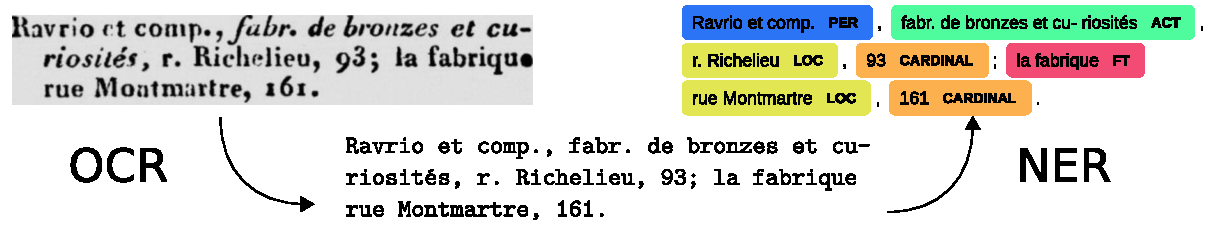
\includegraphics[width=.9\textwidth]{figs/overview-intro.pdf}
    \caption{%
    Overview of the pipeline under study.
    From previously-extracted images of directory entries, 
    we perform OCR and named entity recognition (NER) using different techniques.
    We aim at answering the following questions:
    \emph{How noisy are modern, out-of-the-box OCR systems?}
    \emph{What is the behavior of NER when OCR is noisy?}
    \emph{Can NER be made more robust to OCR noise?}
    }
    \label{<label>}
\end{figure}
\clearpage% force float flush!

\section{Introduction}

% General context + scope limitation
The surge of historical documents digitized by cultural heritage institutions and made publicly available on the Web creates a vast knowledge source that can nourish numerous applications in the fields of social sciences, environmental studies or education.
Most of these documents are texts, either printed or handwritten.
To make the content of these documents searchable and usable by everyone, the texts engraved within them needs to be extracted through optical character recognition (OCR). 
However, OCRed texts are not sufficient to build a high level, semantic view of a collection of documents. A second step thus aims at recognizing in these texts the pieces of information most likely to be searched for by users, such as named entities (people, organizations, dates, places, etc.). Indeed, being able to properly tag text tokens unlocks the ability to relate entities, and provide colleagues from e.g. digital humanities with databases ready for exploitation.

Being active research topics, OCR and named entity recognition (NER) are still difficult tasks when applied to historical text documents.
OCR approaches used for modern documents are likely to struggle even on printed historical documents due multiple causes related to text readability (low resolution scans, inconsistent printing rules, artifacts, show-through), document complexity (intricate and versatile page layout, use of ancient fonts \& special glyphs) and the variability inherent to the huge diversity of historical sources.
\bertrand{ajouter une ref.}
On the other hand, NER approaches developed for modern texts suffer from the time gap between the contemporary entities and the entities mentioned in older texts and from the errors introduced into the text by the OCR step.\nathalie{ajouter une ref}

In this article we focus on a peculiar category of historical printed books: the city trade directories of Paris from the XIX\textsuperscript{th} century (1801 - 1854).
They contain hundred-pages long lists of people, along with their activity and their address, so much valuable fine-grained knowledge to study the social dynamics of the city over time.
Despite containing roughly the same information, the diversity in layouts, information organization and digitizing quality is significant, which hardens makes OCR and NER quite challenging.

In a recent work to locate potentially polluted urban soils \cite{bell2020automated}, trade directories were leveraged to identify and locate all the gas stations in the city of Providence during the XX\textsuperscript{th} century.
The proposed information extraction pipeline extract texts with OCR, identify directories entries and recognizes business type and address within each entry.
In the same way, we aim at producing structured spatio-temporal data from the Parisian trade directories.
These directories originate from several publishers, their content is organized following different indexing methods (by name, by activity or by address), printed in various layouts, use different fonts.
We therefore investigate several state-of-the-art OCR and NER approaches independently and in combination to assess their usability on the directories corpus.
The contributions of this article are the following:
% Contributions
\begin{enumerate}
    \item review state of the art regarding NER for historical documents (section 2)
    \item dataset (section 3)
    \item list usable techniques (more to evangelize the DAR community) (section 4)
    \item compare their performance under various training set sizes (thus annotation costs) and OCR noise levels (thus OCR choices/luck/availability) (sec. 5 and 6)
    \item suggest smart way to leverage side knowledge like lexicons (FIXME iif this works well, maybe a conclusion instead) \nathalie{pas traité dans nos tests... à mettre en perspective}
\end{enumerate}


